% !TEX root=../../report.tex

\Section{Zustände der Vereinbarung}

Der Ablauf der Eventplanung aus \myref{workflow} ist unter der Voraussetzung des Best-Case geplant worden. Das bedeutet in diesem Fall, dass die angefragten Dienstleister, sowie Gäste die Anfragen akzeptieren beziehungsweise annehmen.

Sowohl der Veranstalter, als auch der Dienstleister können aber die Vereinbarung ablehnen. Wird diese Gegebenheit mitbedacht, vervielfältigen sich die möglichen Zustände der Vereinbarung zwischen dem Veranstalter und dem Dienstleister. Zur besseren Übersicht werden die einzelnen Zustände und ihre jeweiligen Übergänge in einem \gls{uml} Zustandsdiagramm veranschaulicht.

\begin{figure}[ht]
\centering
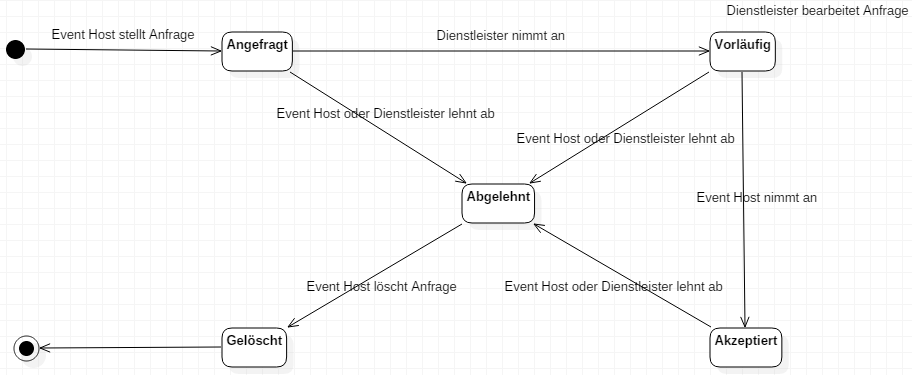
\includegraphics[width=\textwidth]{res/images/AgreementStates.png}
\caption{Zustände der Vereinbarung}
\label{as1}
\end{figure}

Das entstandene Diagramm ist in \myautoref{as1} zu sehen.
Der erste eingenommene Status lautet \enquote{Angefragt}. Er entsteht, indem ein Veranstalter einen Dienstleister zu einem Serviceslot hinzufügt. Nimmt der Dienstleister die Anfrage an, so befindet sich die Vereinbarung im Zustand \enquote{Vorläufig}. Sobald danach der Veranstalter die Vereinbarung akzeptiert, nimmt sie den \enquote{Akzeptiert} Status an und der Vertrag ist zustande gekommen.

Wichtig ist, dass in jedem der möglichen Zustände einer der beiden Vertragspartner ablehnen kann. Durch diese Aktion befindet sich die Vereinbarung im Zustand \enquote{Abgelehnt}. Aus diesem heraus kann die Anfrage von dem Veranstalter gelöscht werden, damit eine neue Zuordnung des Dienstleistungsslots möglich wird.
